\begin{frame}

	\begin{abstract}
		El método de los volúmenes finitos constituye una técnica
		numérica robusta para aproximar la solución de un problema de
		valor inicial frontera de una ley de conservación
		\begin{math}
			\difcp{u}{t}+
			\difcp{f\left(u\right)}{x}=
			0
		\end{math},
		por funciones constantes por partes~\cite[p.~5]{Saeed2025}.
		Este enfoque se basa en discretizar el dominio computacional
		$\Omega\subset\mathbb{R}^{d}$ en una malla compuesta por celdas
		disjuntas
		\begin{math}
			\Omega^{h}=
			\bigcup_{j=1}^{N}
			\Omega_{j}
		\end{math},
		cuya unión cubre el dominio salvo un conjunto de medida nula.
		Para transformar el problema continuo en un sistema algebraico
		discreto, integre la EDP sobre cada celda $\Omega_{j}$.
		Las incógnitas del sistema son aproximaciones del valor medio de
		la solución en cada celda, lo que preserva localmente las
		propiedades de conservación de la EDP.

		\par\vskip\baselineskip\noindent
		{\textbf{Palabras clave}:
			Esquema de Alta Resolución,
			Limitador de flujo,
			Análisis de estabilidad,
			Variación total decreciente.}
		\par\vskip\baselineskip\noindent
		{\textbf{Clasificación Matemática por Temas}:
			35L04,
			35L65,
			35Q35,
			65L12,
			65M06,
			65M12.}
	\end{abstract}

	\pause

	\visible<.(1)>{
		\begin{figure}[ht!]
			\centering
			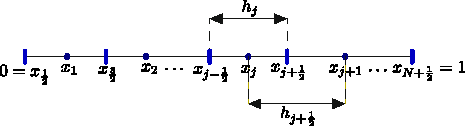
\includegraphics[width=.45\textwidth]{fv1d}
			\caption{
			Malla de volúmenes finitos 1D de $\Omega=\left(0,1\right)$.
			Los nodos de índices fraccionarios
			\begin{math}
				{\big\{x_{j\pm\frac{1}{2}}\big\}}^{N}_{j=1}
			\end{math}
			son los extremos de las celdas
			\begin{math}
				\Omega_{j}=
				\big[
					x_{j-\frac{1}{2}},
					x_{j+\frac{1}{2}}
					\big]
			\end{math}
			cuyo tamaño es $h_{j}$, y los nodos de índices enteros
			\begin{math}
				{\big\{x_{j}\big\}}^{N}_{j=1}
			\end{math}
			son los centros de las celdas.
			Si $x_{0}=-x_{1}$ y $x_{N+1}=2-x_{N}$, entonces $h_{0}=h_{1}$ y
			$h_{N+1}=h_{N}$.
			La distancia entre dos celdas consecutivas es
			\begin{math}
				h_{j+\frac{1}{2}}=
				\frac{1}{2}\left(h_{j}+h_{j+1}\right),
				\forall j=0,\dotsc,N
			\end{math}.
			}
		\end{figure}
	}
\end{frame}
